%************************************************
\chapter{Introduction}\label{ch:introduction}
%************************************************

Fine chemicals manufacturers are under pressure to reduce the cost and environmental impact of their processes. These businesses produce high value chemical products such as pharmaceuticals and agrochemicals, where a regulatory body needs to approve each product and the process used to manufacture it. This approval process can take years and result in millions of dollars in development costs \cite{Prasad2017}. Consequently, reducing cost during product development is a primary target for many fine chemicals manufacturers. Ideally, this would be achieved by "Right First Time" scale-up, where processes can be scaled from the laboratory to manufacturing with minimal effort \cite{Poechlauer2013}. In addition to cost concerns, environmental concerns come from the fact that fine chemicals processes produce the most industrial waste and use the most energy per unit of product among all chemical processes (e.g., commodity, speciality) \cite{Sheldon2018}. Therefore, many fine chemicals companies have committed to making significant reductions in their waste production and energy usage over the next ten years to meet goals set by governing bodies \cite{BASF2020}.

One of the barriers to reducing the cost and environmental impact of fine chemicals development is batch processing (BP).  In BP, each chemical reaction is carried out independently before moving to the next step. BP is used in early stage research to discover chemical routes, and, as shown in Figure \ref{batch_v_flow}, this batch approach is scaled to the pilot plant, where 10-500 kg of new products are manufactured for regulatory approval. Batch processes are notoriously difficult to scale up from the laboratory to the pilot plant. For example, it is not uncommon for a reaction that works perfectly at the laboratory scale to fail in the pilot plant due to insufficient heat and mass transfer in a larger reactor. These "scale-up failures" are costly because the reactants and reagents used in fine chemicals reactions are often expensive. Additionally, multiple batches are usually required in BP, and large volumes of solvent are used to clean the reactors between batches \cite{Lee2016, Sheldon2018}. This explains, in part, why solvents are the main contributor to the environmental waste from fine chemicals processes \cite{Rogers2019}.

\begin{figure}[bt]
  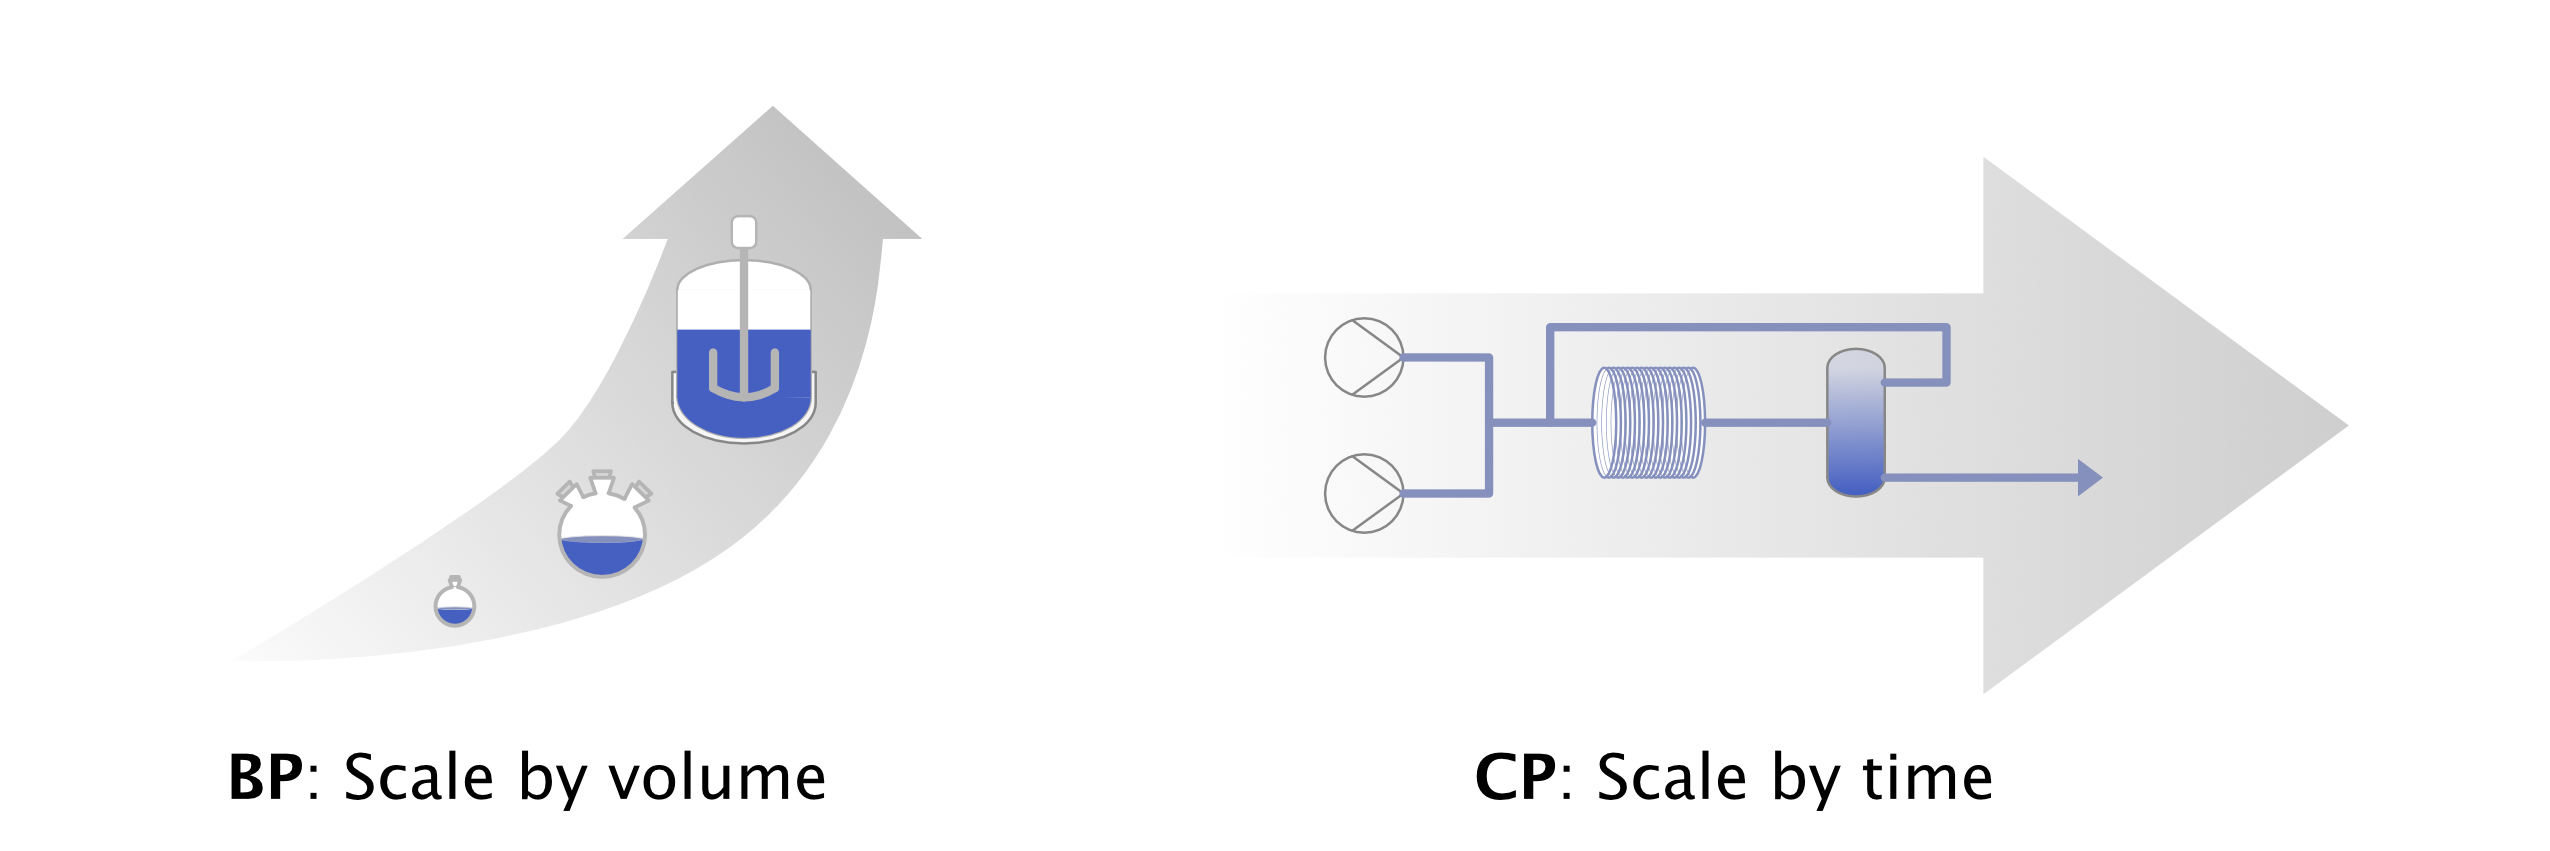
\includegraphics[height=0.2\textheight]{gfx/Chapter01/scale_up_schematic.png}
  \caption{Schematic comparing batch and flow chemistry. Batch processing (BP) achieves scale by increasing volume, while continuous processing (CP) achieves scale by continuous production over time.}
  \label{batch_v_flow}
\end{figure}

Continuous processing (CP) offers a potentially lower cost and more environmentally friendly alternative to BP by integrating multiple steps to form an uninterrupted manufacturing line (see Figure \ref{batch_v_flow}). Material flows continuously between units, so the process can be run for several days without interruption to produce large volumes of material. CP removes the need for cleaning equipment during a campaign, which reduces solvent use significantly \cite{Lee2016}. Furthermore, pilot plant CP equipment is often an order of magnitude smaller than in BP due to its higher space time yield \cite{Elvira2013}. The smaller equipment size decreases CapEx expenditures significantly \cite{Escriba-Gelonch2019} and makes scale-up faster and more reliable due to the pilot plant and laboratory being at nearly the same scale \cite{Cole2019, Rogers2019}. In fact, one of the attractive features of CP is the ability to reduce a several thousand square meter pilot plant facility to a laboratory fume cupboard \cite{Cole2017, Cole2019}.

However, realizing these benefits requires optimized processes. For example, when optimizing chemical reactions for flow, process engineers need to find reaction conditions that balance maximizing throughput and minimizing impurity generation and solvent use. Optimizing reactions at an early stage requires scientists to select continuous (temperature, concentrations, flowrates) and categorical variables (solvent, base, catalyst, ligand), and previous analysis has suggested that many reactions have over 50 million potential conditions \cite{Murray2013}. Thus, simple brute-force screening is not sufficient since experiments are expensive and time-consuming.

Similarly, separations used in flow processes require control systems to maintain high purity separations, even at the laboratory scale. These controllers measure key process parameters and adjust controllable parameters such as valve openings to achieve desired setpoints. Tuning controllers to be both responsive and safe requires significant expertise and time when done manually, and existing automated methods are best suited to large scale manufacturing plants are not efficient when used on live plants. In the case of reactions and separations, scientists have limited capacity to collect experimental data on each task, but historical data exists across multiple tasks.

Therefore, there is a strong need to develop approaches that can quickly optimize flow chemistry processes when only limited experimental data is available. Recently, machine learning has been proposed as a solution to reducing the experimental burden for process development \cite{Taylor2023a}.  However, these techniques either can rely on a large amount of existing data or actively gathering new data.  In other domains, the amount of data required for machine learning has been reduced using transfer learning. 

Transfer learning leverages knowledge gained from one task and applying it to another \cite{Zhuang2021}. In other domains, transfer learning has shown promise for building machine learning that works with small amounts of data. For example, most image classification models are now pretrained on a large dataset of general images, so training on a new classification task only requires a small number of images \cite{He2016}. Similar results have been seen in natural language processing \cite{Brown2020} and even drug discovery \cite{Ramsundar2017}. 

Considering developments in transfer learning, this thesis aims accelerate chemical process development in the pharmaceutical and speciality chemicals industries by reducing the number of experiments required to bring a new process to market. The overarching question of the thesis is as follows:
\begin{displayquote}
Can transfer learning be used to accelerate process development by of separations and reactions by leveraging data from multiple sources? 
\end{displayquote}
Chapter two contains an overview of transfer learning. I review the key concepts underlying transfer learning and demonstrate how transfer learning can be used in the context of the machine learning algorithms applied in this thesis.  The subsequent chapters are split into three parts.

In Part I (chapters three and four), I focus on reaction optimization, an essential part of achieving high efficiency continuous processes. In chapter three, I review the existing literature on automated reaction optimization and introduce Summit, a framework for benchmarking machine learning for reaction optimization.  In chapter four, I demonstrate how a transfer learning technique, namely multitask Bayesian optimization, can accelerate reaction optimization. I present \textit{in silico} benchmarking of multitask Bayesian optimization using Summit and results from collaborative work with experimentalists.

In Part II (chapters five and six), I turn to controller tuning for laboratory distillation columns. Laboratory distillation columns are utilized to separate novel mixtures in regulatory approval campaigns and to ensure that separation of a novel mixture works before investing in building a new large scale distillation column. In chapter five, I review the literature on controller tuning and present an initial failed attempt at using reinforcement learning to tune PID controllers. In chapter six, I present an alternative approach that relies on rigorous dynamic simulation and a transfer learning technique called multifidelity Bayesian optimization.

In Part III (chapters seven and eight), I examine methods for predictive thermodynamics. My interest in this topic came from the challenge of simulating distillation columns for new mixtures, which requires vapor liquid equilibrium (VLE) data. In chapter seven, I introduce \textit{DeepGamma} a method for predicting activity coefficients using deep learning. I show that, in this case, transfer learning does not improve predictions. In chapter eight, I introduce ML-SAFT, a framework for predicting the parameters of the PCP-SAFT equation of state. I show that in this case, transfer learning from simulations to experimental data can improve predictions.

%*****************************************
%*****************************************
%*****************************************
%*****************************************
%*****************************************




